\documentclass[11pt]{article}
\usepackage[top=2.5cm, bottom=2.5cm, left=3cm, right=3cm]{geometry}

\usepackage{graphicx}
\usepackage{fancyhdr}
\usepackage{ETHlogo}
\usepackage[printonlyused]{acronym}
\usepackage{wrapfig}
\usepackage{siunitx}
\usepackage[obeyspaces]{url}
\usepackage[table,dvipsnames]{xcolor}
\usepackage[colorlinks=true, linkcolor=darkgray, urlcolor=RoyalBlue, citecolor=RoyalPurple]{hyperref}
\usepackage{fontawesome}
\usepackage{subcaption}
\usepackage{xparse}
\usepackage{ifthen}
\usepackage{multirow}
\usepackage{tabularx}
\usepackage{todonotes}
\usepackage{upgreek}


\def\thickhrulefill{\leavevmode \leaders \hrule height 1pt\hfill \kern \z@}
\makeatletter
\graphicspath{ {pics/} }
\def\input@path{ {sections/} }
\makeatother
\newfontfamily\ubuntu{Ubuntu}
\newfontfamily\dejavu{DejaVuSans}
\sisetup{detect-weight=true, detect-family=true, product-units=single, range-units=single, range-phrase=$\ \sim\ $, separate-uncertainty=true, exponent-product=\ensuremath{\cdot}}

\setlength{\headheight}{14pt}
\pagestyle{fancy}
\newcommand{\li}{\left|}
\newcommand{\re}{\right|}
\newcommand{\const}{\text{const.}}
\newcommand{\z}{\text}
\newcommand{\terminal}[1]{\colorbox{black}{\textcolor{white}{{\fontfamily{phv}\selectfont \scriptsize{#1}}}}}
\newcommand{\plugin}[1]{\textit{\flq#1\frq}}
\newcommand{\ra}{$\rightarrow$ }
\newcommand{\ar}{\autoref}
\newcommand{\good}[1]{{\usebeamercolor[fg]{title}{\textbf{#1}}}}
\newcommand{\bad}[1]{\textcolor{RedOrange}{\textbf{#1}}}
\newcommand{\dead}[1]{\textcolor{NavyBlue}{\textbf{#1}}}
\newcommand{\cmark}{\good{\ding{51}}}
\newcommand{\xmark}{\bad{\ding{55}}}
\newcommand{\itemfill}{\setlength{\itemsep}{\fill}}
\newcommand{\orderof}[1]{$\mathcal{O}\left(#1\right)$}
\newcommand{\code}[1]{{\footnotesize\dejavu #1}}
\newcommand{\var}[1]{\textcolor{JungleGreen}{#1}}
\newcommand{\meth}[1]{\textcolor{RedOrange}{#1}}
\newcommand{\incl}[1]{\textcolor{YellowGreen!70!RawSienna!100}{#1}}
\newcommand{\str}[1]{\textcolor{MidnightBlue!60!black!100}{#1}}
\newcommand{\tline}[1]{\noalign{\hrule height #1pt}}
\newcommand{\fatwhite}[1]{\multicolumn{1}{c}{\textcolor{white}{\textbf{#1}}}}
\renewcommand{\deg}{$^{\circ}$}
\newcommand{\fpath}[1]{\textbf{\path{#1}}}
\renewcommand\tabularxcolumn[1]{m{#1}}
\newcommand{\alternatecolors}{\rowcolors{2}{YellowOrange!10}{ProcessBlue!10}}
\newcommand{\missfig}[1][.5]{\begin{center} \missingfigure[figheight=#1\textheight,figwidth=#1\textheight, figcolor=white]{}\end{center}}
\newcommand{\caplab}[2]{\ifthenelse{\equal{#1}{nocap}}{}{\caption{#1}}\ifthenelse{\equal{#2}{nolab}}{}{\label{#2}}}
\newcommand{\pic}[3]{\ifthenelse{\equal{#1}{r}}{\includegraphics[height={#2\linewidth}, angle=-90]{#3}}{\includegraphics[width={#2\linewidth}]{#3}}}
%SUBFIG
\DeclareDocumentCommand{\subfig}{O{.45} O{0} m O{n} m O{nocap} O{nolab}}{\begin{subfigure}{#1\linewidth}\vspace*{#2\textheight}\centering\pic{#4}{#3}{#5}\caplab{#6}{#7}\end{subfigure}}
%SUBFIGS
\DeclareDocumentCommand{\subfigs}{O{fig} m m O{nocap} O{nolab}}{\begin{figure}[ht!]\centering\ifthenelse{\equal{#1}{fig}}{}{#1\hspace*{.05\linewidth}}#2\hspace*{.05\linewidth}#3\caplab{#4}{#5}\end{figure}}
%FIG
\DeclareDocumentCommand{\fig}{O{n} m m O{nocap} O{nolab}}{\begin{figure}[ht!]\centering\pic{#1}{#2}{#3}\caplab{#4}{#5}\end{figure}}
% WRAPFIG
\DeclareDocumentCommand{\wrapfig}{O{l} m m O{nocap} O{nolab}}{
	\begin{wrapfigure}{#1}{#2\linewidth}\includegraphics[width={.95\linewidth}]{#3}\caplab{#4}{#5}\end{wrapfigure}}
\DeclareSIUnit\mhzcm{\mega\hertz\per\centi\meter^2}
\DeclareSIUnit\khzcm{\kilo\hertz\per\centi\meter^2}
\DeclareSIUnit\ncm{n\per\centi\meter^2}
\makeatletter

\newcommand*{\version}[1]{\gdef\@version{#1}}
\newcommand*{\@version}{0.0.0}
\newcommand*{\documenttype}[1]{\gdef\@documenttype{#1}}
\newcommand*{\@documenttype}{Documentation}

\renewcommand*{\maketitle}{
\begin{titlepage}

	\begin{figure}
		\begin{minipage}{0.45\linewidth}\flushleft
			\ETHlogo[5cm]
		\end{minipage}
		\hfill
		\begin{minipage}{0.45\linewidth}\flushright
			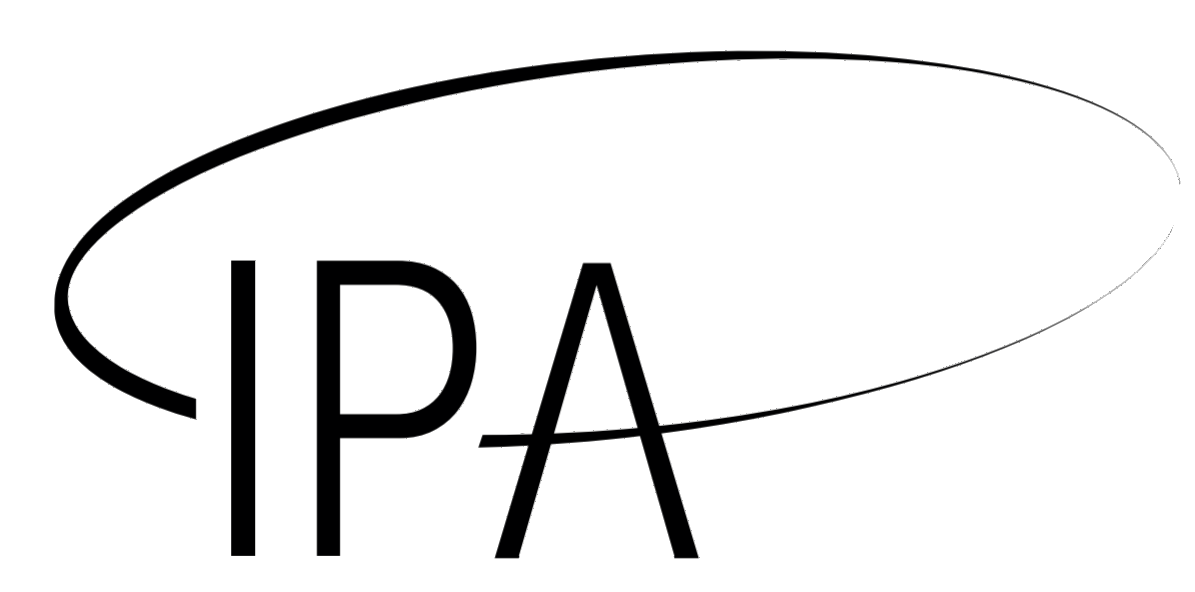
\includegraphics[height=1.5cm]{IPA.png}
		\end{minipage}
		\hrule height 1pt
	\end{figure}\vspace*{.5cm}
	
	\centering
	{\Large\scshape \@documenttype \strut\par}\vspace*{.5cm}
	{\Huge\bfseries\@title\unskip\strut\par}\vspace*{1.5cm}
	{\large\@author\unskip\strut\par}\vspace*{.5cm}
	\begin{abstract}

 During the test of new 3D diamond detectors in PSI beam tests using \SI{260}{\mega\electronvolt} positive pions we measured pulse heights far below the trimmed threshold of the ROCs. Both a diamond 3D detector connected via indium bump bonds as well a standard silicon sensor were measured using the psi46digv21respin ROC and showed the same behaviour. The observed behaviour could could not be reproduced using test signals of the ROC electronics.
	
\end{abstract}






	\vfill
	
	\flushleft
	ETH Z\"urich, Switzerland, \@date \hfill Version \@version

\end{titlepage}}







\documenttype{Documentation}
\title{Low Pulse Heights in CMS Pixel Chips}
\author{Michael Reichmann}
\date{\today}


\makeindex
\begin{document}

% ========== TITLE PAGE WITH ABSTRACT ============
	\maketitle

	\thispagestyle{empty}
	\cleardoublepage\tableofcontents
	\setcounter{page}{0}
	
	
% ========== MAIN PART OF THE DOCUMENT ===========
	\cleardoublepage
	\section{Test Site}

The measurements were taken at the \ac{PSI} beam line PIM1 with the following parameters:
\begin{itemize}
	\item particle type: positive pions
	\item particle momentum: \SI{260}{\mega\electronvolt}
	\item particle fluxes: \SIrange{10}{20000}{\khzcm}
\end{itemize}






	\section{Detectors}

\subsection{Si352}

Standard silicon pixel detector built at \ac{PSI} using the psi46digv21respin \ac{ROC}. The detector is almost nonirradiated and has just seen radiation during beam tests.

\subsection{3D Diamond Detector - II6-B6}

The detector is made out of \ac{pCVD} diamond, has a thickness of \SI{\sim500}{\micro\meter} and has \SI{50x50}{\micro\meter} 3D pixel cells. In order to match the pixel pitch of the CMS pixel chip (\SI{150x100}{\micro\meter}) \SI{3x2}{cells} were ganged together and connected to the same bump bond.\par
A picture of the final detector is shown in \ar{fig:3d}. Since the diamond detector has only a size of \SI{\sim4x4}{\mm} it is only connected to a part of the bigger \ac{ROC}. 
\fig{.5}{3D}[3D diamond detector on a CMS pixel chip][fig:3d]




	\section{Measurements}

\subsection{Setup \& Readout}
\fig{.7}{setup}[ETH Telescope setup with one motherboard and three planes][fig:1]
A demo setup of a ETH Telescope module is shown in \ar{fig:1}. The detectors are glued and wirebonded to a standard carrier-board and then connected to a custom Adaptor-plane via the SAMTEC connector. These Adaptor planes are then plugged into a motherboard which directly connects to the \ac{DTB}.\par
The test boards are operated with the pixel-dtb-firmware dtb\_v4.2 using the pXar-core libraries.

\subsection{Preparation}
Both \acp{ROC} of the diamond detector was trimmed to a threshold of \SI{30}{vcal} and the one of the silicon to \SI{32}{vcal} using the standard trimming algorithm of the pXar GUI in the beam area at ambient temperature without cooling. The pulse-height \acp{DAC} \code{phoffset} and \code{phscal} were then adjusted to achieve linear response of the adc vs vcal in the desired range. The according dacParameter.dat files are shown in \ar{sec:app} (Appendix).

\subsection{Hit Maps}
\subfigs{\subfig{.8}[r]{HM-B6}[Hit map of the diamond detector. Dark blue area corresponds to area where the detector has no readout columns and is only connected to the bump bond. The white area is masked by the chip.]}{\subfig{.8}[r]{HM-S}[Hit map of the silicon detector. The profile corresponds to the shape of the trigger area.\vspace{36pt}]}

\subsection{VCAL Distributions}
Using the phCalibration.dat files yields the following vcal distributions.
\subfigs{\subfig{.8}[r]{VD-B6}[Diamond]}{\subfig{.8}[r]{VD-S}[Silicon]}
Even though more dominant in the diamond device both chips show parts of the distribution that are below a the tuned threshold. It even appears as if there is an additional Gaussian contribution around exactly zero vcal. The \acp{MPV} are exactly in the expected positions considering the deposited energies in the detectors.

\subsection{Low Pulse Height Hit Maps}
The position of the hits with a pulse height below the tuned threshold seems more dominant certain pixels but is distributed over the full chip.
\subfigs{\subfig{.8}[r]{CMC-B6}[Diamond]}{\subfig{.8}[r]{CMC-S}[Silicon]}
	
% ========== APPENDIX STUFF ======================
	\newpage
\section*{Appendix}\label{sec:app}

\begin{table}[h!]
	\begin{minipage}{.45\textwidth}\centering
		\begin{tabular}{rrl}
			\textbf{Nr.} 	& \textbf{Name}		& \textbf{Value} 					\\\noalign{\hrule height 1.3pt}
			1							& vdig						& 6	\\
			2							& vana						& 74	\\
			3							& vsh							& 30	\\
			4							& vcomp						& 12	\\
			7							& vwllpr					& 150	\\
			9							& vwllsh					& 150	\\
			10						& vhlddel					& 250	\\
			11						& vtrim						& 130	\\
			12						& vthrcomp				& 108	\\
			13						& vcolorbias			& 30	\\
			17						& phoffset				& 185	\\
			19						& vcomp\_adc			& 50	\\
			20						& phscale					& 65	\\
			22						& vicolor					& 100	\\
			25						& vcal						& 200	\\
			26						& caldel					& 152	\\
			253						& ctrlreg					& 0	\\
			254						& wbc							& 100	\\
			255						& readback				& 0	\\
		\end{tabular}
		\caption{dacParameters.dat for II6-B6}
	\end{minipage}
	\hfill
	\begin{minipage}{.45\textwidth}\centering
		\begin{tabular}{rrl}
			\textbf{Nr.} 	& \textbf{Name}		& \textbf{Value} 					\\\noalign{\hrule height 1.3pt}
			1							& vdig						& 6	\\
			2							& vana						& 90	\\
			3							& vsh							& 30	\\
			4							& vcomp						& 12	\\
			7							& vwllpr					& 150	\\
			9							& vwllsh					& 150	\\
			10						& vhlddel					& 250	\\
			11						& vtrim						& 145	\\
			12						& vthrcomp				& 106	\\
			13						& vcolorbias			& 30	\\
			17						& phoffset				& 220	\\
			19						& vcomp\_adc			& 50	\\
			20						& phscale					& 100	\\
			22						& vicolor					& 100	\\
			25						& vcal						& 200	\\
			26						& caldel					& 101	\\
			253						& ctrlreg					& 0	\\
			254						& wbc							& 100	\\
			255						& readback				& 0	\\
		\end{tabular}
		\caption{dacParameters.dat for Si352}
	\end{minipage}
\end{table}

% 	\newpage
% 	\pagenumbering{Roman}
% 	\listoffigures
% 	\listoftables
	\newpage
\section*{List of Acronyms}
\begin{acronym}[Bash]
	\acro{IDE}{integrated development environment}
	\acro{DIY}{do-it-yourself}
	\acro{USB}{Universal Serial Bus}
	\acro{I/O}{input/output}
	\acro{GND}{ground}
	\acro{RST}{reset}
	\acro{PWR}{power}
	\acro{IC}{integrated circuit}
	\acro{PCB}{printed circuit board}
	\acro{VCC}{voltage common collector}
	\acro{OS}{operating system}
	\acro{PTC}{positive temperature coefficient}
	\acro{NTC}{negative temperature coefficient}
	\acro{ADC}{analogue-to-digital converter}
	\acro{BJT}{bipolar junction transistor}
	\acro{PWM}{pulse width modulation}
	\acro{PID}{proportional–integral–derivative}
	\acro{RPM}{revolutions per minute}
	\acro{PUC}{pixel unit cell}
	\acro{ROC}{readout chip}
	\acrodefplural{ROCs}{readout chips}  
	\acro{TBM}{token bit manager}
	\acro{UB}{ultra black}
	\acro{B}{black}
	\acro{CMS}{Compact Muon Solenoid}
	\acro{LHC}{Large Hadron Collider}
	\acro{HL-LHC}{High-Luminosity-LHC}
	\acro{CERN}{European Organization for Nuclear Research}
	\acro{DAC}{digital to analogue converter}
	\acro{ADC}{analogue to digital converter}
	\acro{LD}{last DAC}
	\acro{DTB}{digital test board}
	\acro{ATB}{analogue test board}
	\acro{ETH}{Eidgen{\"o}ssische Technische Hochschule}
	\acro{FPGA}{Field Programmable Gate Array}
	\acro{PSI}{Paul Scherrer Institut}
	\acro{HIPA}{High Intensity Proton Accelerator}
	\acro{HV}{high voltage}
	\acro{TTL}{Transistor-Transistor-Logic}
	\acro{PLL}{phase-locked loop}
	\acro{FIFO}{First In - First Out}
	\acro{HAL}{hardware abstraction layer}
	\acro{API}{application programming interface}
	\acro{GUI}{graphical user interface}
	\acro{CLI}{command line interface}
	\acro{DAQ}{data acquisition}
	\acro{CPU}{central processing unit}
	\acro{PG}{pattern generator}
	\acro{I2C}[I$^{2}$C]{Inter-Integrated Circuit}
	\acro{DUT}{device under test}
	\acro{TCP}{Transmission Control Protocol}
	\acro{TU}{trigger unit}
	\acro{COM}{centre of mass}
	\acro{PSB}{Proton Synchrotron Booster}
	\acro{PS}{Proton Synchrotron}
	\acro{SPS}{Super Proton Synchrotron}
	\acro{ALICE}{A Large Ion Collider Experiment}
	\acro{ATLAS}{A Toroidal LHC Apparatus}
	\acro{LHCb}{Large Hadron Collider beauty}
	\acro{LHCf}{ Large Hadron Collider forward}
	\acro{TOTEM}{TOTal Elastic and diffractive cross section Measurement}
	\acro{SUSY}{supersymmetry}
	\acro{HCAL}{hadronic calorimeter}
	\acro{ECAL}{electromagnetic calorimeter}
	\acro{CTR}{calibrate trigger reset}
	\acro{MIP}{minimum ionising particle}
	\acrodefplural{MIPs}{minimum ionising particles}
	\acro{PM}{photo multiplier}
	\acro{TLU}{trigger logic unit}
	\acro{PH}{pulse height}
	\acro{DC}{double column}
	\acro{DESY}{Deutsches Elektronen-Synchrotron}
	\acro{RAM}{Random-Access Memory}
	\acro{PCB}{printed circuit board}
	\acro{PLT}{Pixel Luminosity Telescope}
	\acro{RPC}{remote procedure calls}
	\acro{CVD}{Chemical Vapour Deposition}
	\acro{pCVD}{poly-crystalline Chemical Vapour Deposition}
	\acro{scCVD}{single-crystal Chemical Vapour Deposition}
	\acro{sc}{single-crystal}
	\acro{p}{poly-crystalline}
	\acro{BCM}{Beam Condition Monitor}
	\acrodefplural{BCMs}{Beam Condition Monitors}
	\acro{BLM}{Beam Loss Monitor}
	\acrodefplural{BLMs}{Beam Loss Monitors}
	\acro{DBM}{Diamond Beam Monitor}
	\acro{ToF}{time-of-flight}
	\acro{IP}{interaction point}
	\acro{CCD}{charge collection distance}
	\acro{MFP}{mean free path}
	\acro{OSU}{Ohio State University}
	\acro{SNR}{Signal to Noise Ratio}
	\acro{MPV}{Most Probable Value}
\end{acronym}
	
% ========== BIBLIOGRAPHY ========================
% \newpage
% \bibliographystyle{plain}
% \bibliography{refs}

\end{document}
